
% Template for a Computer Science Tripos Part II project dissertation
\documentclass[12pt,a4paper,twoside,openright]{report}
\usepackage[pdfborder={0 0 0}]{hyperref}    % turns references into hyperlinks
\usepackage[margin=25mm]{geometry}  % adjusts page layout
\usepackage{graphicx}  % allows inclusion of PDF, PNG and JPG images
\usepackage{verbatim}
\usepackage{docmute}   % only needed to allow inclusion of proposal.tex
\usepackage[utf8]{inputenc}
\usepackage[T1]{fontenc}
\usepackage{tabularx}
\usepackage{ragged2e}
\newcolumntype{Y}{>{\RaggedRight\centering\arraybackslash}X}
\usepackage{booktabs}

\raggedbottom                           % try to avoid widows and orphans
\sloppy
\clubpenalty1000%
\widowpenalty1000%

\renewcommand{\baselinestretch}{1.1}    % adjust line spacing to make
                                        % more readable

\begin{document}

\bibliographystyle{plain}


%%%%%%%%%%%%%%%%%%%%%%%%%%%%%%%%%%%%%%%%%%%%%%%%%%%%%%%%%%%%%%%%%%%%%%%%
% Title



\pagestyle{empty}

%\rightline{\LARGE \textbf{}}

%\vspace*{30mm}
\begin{center}
\begin{Huge}
Part II Project\\
\textbf{Constructing 3D Models from Image Sequences} \\[5mm]
Ilinca Gabriela Sorescu \\
\end{Huge}
%\linebreak[5]
\vspace*{10mm}
\centerline{
\includegraphics[scale=0.2]{figs/Newnham_crest.png}}
\Large Newnham College \\
\vspace*{65mm}
\large \today % today's date
\end{center}

%%%%%%%%%%%%%%%%%%%%%%%%%%%%%%%%%%%%%%%%%%%%%%%%%%%%%%%%%%%%%%%%%%%%%%%%%%%%%%
% Proforma, table of contents and list of figures

\pagestyle{plain}

\chapter*{Proforma}

{\large
\begin{tabular}{ll}
Name:               & \bf Ilinca Gabriela Sorescu                       \\
College:            & \bf Newnham College                               \\
Project Title:      & \bf Constructing 3D Models from Image Sequences   \\
Examination:        & \bf Computer Science Tripos -- Part II, July 2015  \\
Word Count:         & \bf  \\
Project Originator: & I. G. Sorescu                     \\
Supervisor:         & Karina Palyutina                  \\ 
\end{tabular}
}



\section*{Original Aims of the Project}




\section*{Work Completed}

All that has been completed appears in this dissertation.

\section*{Special Difficulties}
None.

\newpage
\section*{Declaration}

I, Ilinca Gabriela Sorescu of Newnham College, being a candidate for Part II of the Computer Science Tripos, hereby declare
that this dissertation and the work described in it are my own work,
unaided except as may be specified below, and that the dissertation
does not contain material that has already been used to any substantial
extent for a comparable purpose.

\bigskip
\leftline{Signed}

\medskip
\leftline{Date}

\tableofcontents

\listoffigures

\newpage

%%%%%%%%%%%%%%%%%%%%%%%%%%%%%%%%%%%%%%%%%%%%%%%%%%%%%%%%%%%%%%%%%%%%%%%
% now for the chapters

\pagestyle{headings}

\chapter{Introduction}
The term 3D reconstruction refers to the process of capturing the shape and appearance of real objects.\\
The aim of this project is to undertake the design and implementation of a system which reconstructs the surface of the object from a sequence of photos.\\
\linebreak
This chapter will explore the motivation for this project along with some of the related work done in this field. 

\section{Motivation}
This section will introduce the reader to the wide range of applications of the proposed system and explain why more work needs to be done in the field of 3D reconstruction.\\
\linebreak 
The ability to construct digital models of the objects we might encounter on a day-to-day basis has proven to be a valuable asset with applications in many different areas. Here are a few examples of such applications:
\begin{itemize}
\item medicine: recent efforts have made significant leaps towards making 3D printing of organs a reality. In order to create a functional replica of a sick organ we must first produce a digital model of the organ which needs to be replaced. 
\item manufacturing process: 3D models can expedite the design process of the next prototype of a product or help to reverse-engineer the development of a given object.   
\item restoration: digital models can facilitate the restoration process of objects with cultural importance. In addition to this, entire museum collections could be made available online as 3D galleries.  
\item scientific analysis: the digital analysis of a 3D map of the terrain in a specific area could lead to scientific breakthroughs in geology.
\end{itemize}
In some of the cases outlined above systems which serve a similar purpose to the one described in this document are already in use. Nonetheless, it has become apparent that many more industries could greatly benefit from the use of such a system. Their failure to adopt this strategy suggests that the systems available thus far are either incompatible or too expensive. Either way, it is clear that more development needs to be done in this area. \\  
\linebreak
The technology currently used for constructing 3D models is based, in most cases, on the use of 3D scanners. What follows is a justification of the need for a general-purpose 3D modeling system which is based on a sequence of pictures, thus superseding the use of specialized hardware:
\begin{itemize}
\item 3D scanners are expensive
\item some of the possible applications of 3D reconstruction go beyond the current range of applicability of 3D scanning. 
\item pictures can be taken with any digital camera, including the ones embedded in mobile phones. Since most people have their mobile phones with them at all times, this means that the users do not have to foresee the need to create a 3D reconstruction. This is especially useful in making 3D reconstruction available for home users which could lead to the development of a new direction in video gaming.
\end{itemize}
For the reasons outlined above, exploring a cheaper alternative to constructing 3D models based on data acquired with 3D scanners is a worthwhile effort. This document describes my attempt to construct such a system. 

\section{Challenges}
In the last section I tried to convince the reader that the world would benefit from a more widespread usage of 3D reconstruction. The purpose of this section is to explain why, in spite of all of its advantages, 3D reconstruction still has a restricted range of applicability today. \\
\linebreak
Computer vision, the scientific discipline concerned with making computers understand the visual world of humans, is still in its infancy, according to many experts in this field. \\
The main reason for this lack of expertise is that vision is an \textit{inverse problem}: we are seeking to create a mapping from a two dimensional space to a three dimensional one. Clearly, we are given insufficient information to fully specify the solution \cite{Szeliski+2011}.\\
\linebreak
Like most inverse problems, 3D reconstruction is an ill-posed problem because it disobeys the last two conditions of \textit{Hadamard's criteria} \cite{+2008}:
\begin{itemize}
\item There is a solution.
\item The solution is unique.
\item The solution depends continuously on the initial conditions.
\end{itemize}
Each of the disobeyed conditions adds to the difficulty of the task:\\
\begin{itemize}
\item If there are multiple possible solutions for an inherent part of the task one must be able to identify which factors make a solution more probable than another. In the case of 3D reconstruction, determining the depth attributes of the scene can have more than one solution. The reasons for this will be discussed later.
\item If the third condition is disobeyed, the solution is likely to be very error-prone.
\end{itemize}
The complexity of an ill-posed problem is very easy to underestimate. However, in some respects, providing an exact solution to such a problem is an \textit{AI-complete} task.\\
The working solutions of ill-posed problems in the field of computer vision attempt to go around this issue by approximating the result rather than determining it, or by placing some limitations on the input data. Unfortunately, in the case of 3D reconstruction, the result is still noticeably distorted in some cases.\\
\linebreak
The ill-posed nature of the task is not the only complication which was expected to arise. Other factors which increased the risk of the undertaking are having to rely on the performance of external libraries any my own inexperience with projects of this scale. 

\section{Related work}
This section serves to present some of the work done in the field of 3D reconstruction and to discuss its techniques and results in the light of this project.\\
\linebreak
A list of 3D reconstruction software can be found at \url{http://en.wikipedia.org/wiki/Comparison_of_photogrammetry_software}. Most of the entries in this list do not fully reflect the aims of this project either because they make use of 3D scanners or other specialized hardware or because they don't provide support for automatic modeling. Nonetheless, the accuracy with which such software reconstructs an object is an important factor to consider when deciding whether this project should be considered a success.\\
\linebreak
\begin{figure}
\centerline{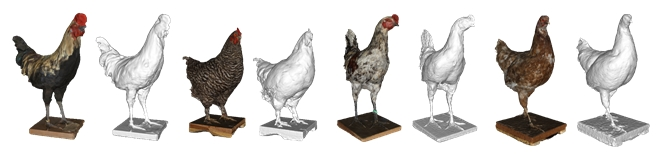
\includegraphics[scale=0.8]{figs/CHICKENS.jpg}}
\caption{Results in the field of 3D reconstruction. The digital models of chickens are obtained using the web-based tool ARC3D. These models were constructed as part of the iMinds INSTANCE project.}
\end{figure}
Out of the software presented in the link above, the tool which best resembles the aims of this project is Ku Leuven's ARC3D\footnote{http://homes.esat.kuleuven.be/~visit3d/webservice/v2/}. This impressive web-based software is a free, fully-automatic tool for extracting a 3D model from a sequence of images. Its 3D photo gallery\footnote{http://homes.esat.kuleuven.be/~konijn/3d/} unveils a series of life-like models, some of which were even used in order to print replicas of the initial object.\\
\linebreak
ARC3D bases its computation on the notion of dense reconstruction\cite{tingdahl_lncs_11}. This is more powerful than the approach described in the following chapters of this document because it aims to estimate the depth of the scene at every pixel of the image, not only at a few relevant locations. Albeit dense reconstruction leads to better results, the risks involved in understanding, planning and implementing it in time make it an unfeasible approach for the core of this project. Due to the use of sparse reconstruction, the results of this project are expected to be noisier than those of ARC3D. 


\chapter{Preparation}
The original aims of this project, as presented in the project proposal, amount to a very broad description of the task to be undertaken. However, the successful completion of a challenging project of this scale requires a great deal of careful planning. This chapter presents some of the aspects which factored into planning the execution of a system which aims to reconstruct the scene from a sequence of images.\\
\linebreak
The chapter starts off by identifying the requirements of the system, then it proceeds to describe the structure of the project as it has developed from these requirements. What follows is a description of the tools and methodologies involved in the development of this project. 

%\subsection{Stereo vision and stereo correspondence}
%Stereo vision is the process of recovering depth information from a pair of 2D %projections of the a scene as seen from two different viewpoints.\\ 
%\textit{Although in this project more than two viewpoints will be used, the task of recovering 3D data from multiple 2D projections is difficult for the same fundamental reason as stereo vision is. For simplicity, this section will analyze the difficulties which arise from attempting to recover a 3D scene from two images.} \\

\section{System Overview and Requirement Analysis}
This section aims to identify the requirements which must be fulfilled by any successful implementation of the system described in this document.\\
In addition to serving as a criterion in deciding whether the project is successful or not, such an analysis is an inherent part of the early stages of the project because it provides a base for planning the implementation and for structuring the system.\\
\linebreak
This section presents a broad overview of the system and then proceeds to identify the functional requirements of the project.
\subsection{Overview of the Project}
In order to achieve the purposes of this project, a working system which constructs a three-dimensional model based on a sequence of images must be put together. \\
After analyzing the input images, the system aims to build a set of points which are considered to be lying on the surface of the input object. These points are then connected together in order to construct a polygon mesh. The newly-constructed surface is then exported as a \textbf{PLY} file.\\
\subsection{Functional Requirements}
\begin{samepage}
Table 2.1 summarizes the goals of this project. The information displayed in this table is in conformity with what was presented in the project proposal, but it provides a lower-level overview of the functional components of the system.\\
For each of the functional components listed above the table specifies the priority within the system and provides an estimate of the difficulty and risk expected to arise in the implementation of that component. Because there is a substantial amount of risk involved in carrying out this project, careful consideration was given to estimating the risk of each functional unit. The main  factors which were taken into account in determining the risk of a task are:
\begin{itemize}
\item whether the task is ill-posed. For reasons presented in the introductory chapter of this document, the main source of risk in this project comes from the ill-posed nature of the underlying problem.
\item whether the outcome is expected to need further refinement. Post-processing is commonly used in order to correct the result of an error-prone computation.
\item whether it involves solving complicated mathematical equations. I consider this to be a source of risk because typically such computations are harder to debug and imply a loss of precision.
\end{itemize}     
\begin{center}
\begin{table}
\begin{tabularx}{\textwidth}{@{} Y c c c @{}} % use 'Y' for first column
\toprule
\textbf{Functional Requirements} & \textbf{Priority} & \textbf{Difficulty} & \textbf{Risk}\\ \hline
\midrule
Build a tool for generating pictures from a 3D model                    &   High       &     Low      &   Low \\ \hline \addlinespace
Implement a tool which constructs a point cloud using triangulation   &   High       &     Medium      &   High \\ \hline \addlinespace
Improve stereo correspondence using an epipolar filter                  &   Medium       &     High      &   High \\ \hline \addlinespace
(optional)Implement other filters to build a better point cloud         &   Low       &     Medium      &   Medium \\ \hline \addlinespace
Construct the surface from the resulting point cloud                    &   Medium       &     High      &   High \\ \hline \addlinespace
Add functionality to export the surface as .PLY                         &   Low       &     Low      &   Low \\ 
\bottomrule
\end{tabularx}
\caption{Functional requirements} 
\label{table:nonlin}
\end{table}
\end{center}
\end{samepage}
It is important to note that this system only aims to build the polygon mesh of the surface. Therefore I regarded capturing the texture and shading of the scene non-requirement. The system can be extended later to include this functionality.\\
I am also planning to build the system as one or multiple console applications, hence discarding the need to build a user interface. The applications will display a help message containing information about the tool's intended purpose and usage.

\section{The Main Components of the System}
After a careful evaluation of its required functionality, the system was split into these logically-different entities:
\begin{itemize}
\item \textbf{Image Generator}
Given a three-dimensional object as input, the picture generator produces a specified number of digital pictures of that object, along with the corresponding locations from which the pictures have been taken. 
\item \textbf{Point Cloud Constructor}
The point cloud constructor aims to generate points which lie on the surface of the input model in the three-dimensional space. 
\item \textbf{Surface Reconstructor}
The surface reconstructor converts the point cloud constructed by the previous module into a triangular mesh. The resulting representation of the surface is exported into a \textit{.PLY} file.
\item \textbf{Evaluation Module}
The purpose of the evaluation module is to analyze the performance of the point cloud constructor and of the surface reconstructor by comparing their result to the original model. \\
\end{itemize}
\begin{figure}
\centerline{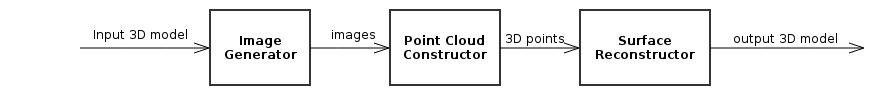
\includegraphics[scale=0.7]{figs/overview.png}}
\caption{An overview of the system}
\end{figure}


\section{Dependency Analysis}
\begin{figure}
\centerline{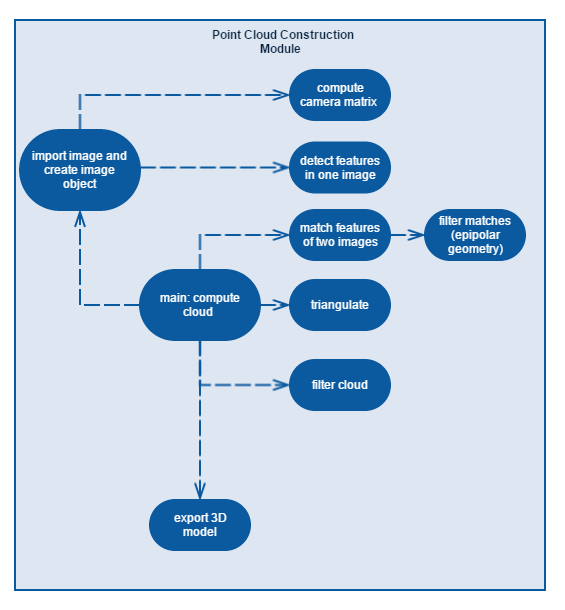
\includegraphics[scale=0.75]{figs/dependencies.png}}
\caption{Dependencies between different units of the project}
\end{figure}


\section{Choice of Tools}
\subsection{Programming Languages}
\subsection{Libraries}
\begin{figure}
\centerline{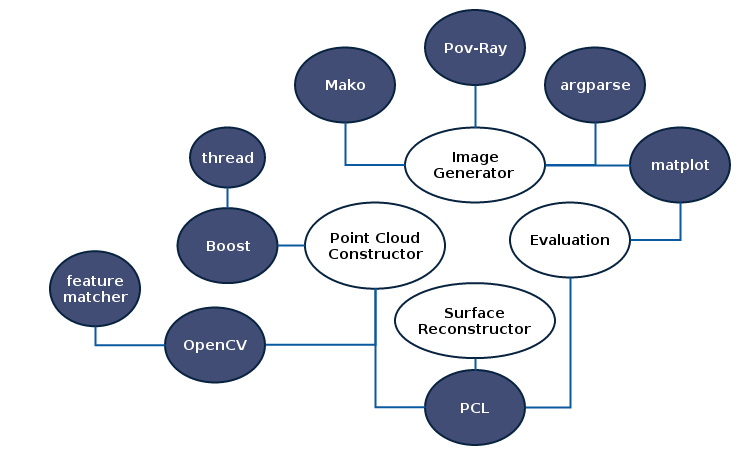
\includegraphics[scale=0.8]{figs/libraries.png}}
\caption{The libraries and other external software used in the development of this project. The white nodes represent modules of the project.}
\end{figure}
\subsection{The Ray Tracer} 
The purpose of one of the main parts of the system, the image generator, is to produce an alternative to photographs of a real-life object. The performance of the system will be evaluated based on what it produces when applied to this computer-generated input. Therefore, for this evaluation to be sound, the input used must be a near photo-realistic representation of the object.\\  
\linebreak
A ray tracer accomplishes just that: given a three-dimensional description of a scene, it creates a digital image of that scene as seen from a predefined location. Many of the ray tracers available yield pictures which are realistic enough for the purposes of this project. \\   
I used \textbf{The Persistence of Vision RayTracer}, or \textbf{POV-Ray}, because it generates images from a text-based scene description. This gives me a lot of flexibility in setting the location of the camera and the light conditions of the scene for every snapshot in turn directly from the script.\\
Another great advantage of \textbf{POV-Ray}\footnote{http://www.povray.org/} is that it comes with a free object collection (\url{http://objects.povworld.org/}). I can evaluate the results of my system on any one of these instead of having to create my own objects.\\
Convenience factors aside, \textbf{POV-Ray} is one of the highest-quality free ray tracers available.\footnote{http://hof.povray.org/}
\subsection{The programming environment}
\subsection{Versioning control}
\section{Software engineering techniques}
\section{Summary}

\chapter{Implementation}
This chapter outlines and provides explanation for some of the specific decisions involved in the design and implementation of the system described in this document. It begins by presenting the purpose of the different modules that the system consists of and the interactions between them and then proceeds to explain each of the modules in more detail. The last section presents a summary of the important points made in this chapter.

\section{Overview of the System}
Reiterate in short what was in prep in overview
\textit{Note on the division into prototypes: As specified in the project proposal, the development of the system was conducted in a prototyped fashion. This chapter presents the final version without discriminating between different prototypes. For a description of the differences between the prototypes see section !! of the evaluation chapter.}

\section{The Image Generator}
As described in the previous section, this module produces a sequence of digital snapshots of a given three-dimensional object as seen from different locations in space. \\
Perhaps the most important aim of this project is to decide whether it would be practical to implement a low-cost system for creating digital representations of real-life objects based on pictures instead of using three-dimensional scanners. Therefore it might seem a bit odd that such a module is needed at all as it is restricting the system's interaction with the outside world. This section aims to explain why such an input generator is used and provide a detailed overview of its intended usage. 
\subsection{The role it plays in the system}
Complex measurements and calculations must be performed in order to determine the accuracy with which the output of the system resembles the real-life object used as input. To avoid this complexity, the input of the system was changed from a sequence of photographs of an object acquired using a hand-held camera to a sequence of digital snapshots of a preexisting three-dimensional model. This is a natural first-step to be taken in deciding whether such a system would yield a reliable representation because it enables one to evaluate the results by comparing the output directly to the input model. More on this topic in the evaluation chapter.\\
Here are some additional advantages of using digital snapshots instead of photos: 
\begin{enumerate}
\item there is no need to worry about camera calibration.
\item the configuration of the scene is very easy to change (e.g.\ the location and orientation of the light sources, the number of snapshots taken, etc.). This is a very important advantage in determining the limiting conditions in which the output is accurate.
\item the input generator can produce a lot of snapshots effortlessly and record the locations from which they were taken.
\item no human assistance is needed in evaluating the system.
\end{enumerate}
The system can be extended to take real photographs as input simply by adding a calibration module.

\subsection{Usage}
This module is executed as a console application. The user must specify the following parameters:
\begin{itemize}
\item \textbf{Filename} The name of (and relative path to) the input object. This must be an include file for \textbf{The Persistence of Vision Raytracer (POV-Ray)} and have the extension \textit{.inc}. The input file is assumed to meet the conditions outlined below:
	\begin{enumerate}
		\item the file defines only one object.
		\item the object defined is included in the scene. For better results it should be placed in the vicinity of the origin.
		\item the scene defined in the file mustn't contain any lights or cameras.
		\item no run-time errors are produced as a result of attempting to render the file using \textbf{POV-Ray}. 
		\item the file doesn't contain any instruction whose purpose is to redefine the length of the units used to something other than the standard \textbf{POV-Ray} units. 
	\end{enumerate}    
\item \textbf{N} The number of snapshots to be taken. This can be any integer greater than 3.
\item \textbf{R} The radius of the sphere considered. The following condition must be fulfilled by \textbf{R}: If you were to look towards the origin through air (using no distorting lenses) from any point at a distance \textbf{R} from the origin you would see the whole object. Here, the origin refers to the origin of the \textbf{POV-Ray} coordinate system and the distance is measured in \textbf{POV-Ray} units.  (for more details on the \textbf{POV-Ray} coordinate systems see \url{http://www.povray.org/documentation/view/3.6.1/15/})
\end{itemize}


\subsection{Language and libraries}
The image generator was implemented using Python. The main factor involved in this decision was the availability of a lightweight library for dealing with templates. I used \textbf{Mako} (\url{http://www.makotemplates.org/}) in order to create \textit{.pov} files from the template \textit{povTemplate.mako}: 

\begin{verbatim}
#include "${filename}"
#include "colors.inc"

light_source { <100, 100, 100> color rgb<1, 1, 1> }

camera {
          location <${", ".join(str(x) for x in camera)}>
          look_at <0, 0, 0>
       }
\end{verbatim} \\

\textbf{Mako} enables the programmer to control the value of the variables (marked with \$) from the Python script. \\
The \textit{.inc} file which defines the input model is included in the first line of the template. \\
I chose to use this approach because it is a painless and straightforward way to control the location of the camera and the light conditions of the scene regardless of the input model used. 

\subsection{Effect and output}
Given the name of the input file, the number of snapshots to be produced(\textbf{N}) and the radius of the sphere considered(\textbf{R}), the image generator determines \textbf{N} points uniformly distributed on the surface of the sphere of radius \textbf{R} centered in origin. These \textbf{N} points represent the locations from which the snapshots will be taken. For each of these camera locations a new \textit{.pov} file will be generated from the \textbf{Mako} template as described in the previous section. Note that the camera is always pointing towards the origin. \\
The \textit{.pov} files are rendered using \textbf{POV-Ray} to create the desired snapshots.

\section{The Point Cloud Constructor}
Given a sequence of snapshots, the point cloud constructor finds correspondences between pairs of snapshots and uses these correspondences to determine the three-dimensional position of points located on the surface of the object.   
\subsection{Libraries}
\subsection{Language choice}
\subsection{Point Cloud Constructor (class)}
\subsection{Image (class)}
\subsection{Feature Matcher (class)}
\subsection{Additional filters}
\subsection{Improving performance}

\section{The Surface Reconstructor}

\section{Model Visualizers}

\section{The Evaluation Module}
This module consists of independent pieces of code which serve the purpose of evaluating the performance of the other modules. It is used in order to automatically plot the accuracy of the resulting representation under different conditions by systematically varying the input arguments of the point cloud constructor and repeatedly rerunning  it to acquire data. 

\section{Summary} 
In this section the user became  acquainted with the internal workings of the system.  


\chapter{Evaluation}


\chapter{Conclusion}


%%%%%%%%%%%%%%%%%%%%%%%%%%%%%%%%%%%%%%%%%%%%%%%%%%%%%%%%%%%%%%%%%%%%%
% the bibliography
\addcontentsline{toc}{chapter}{Bibliography}
\bibliography{refs}

%%%%%%%%%%%%%%%%%%%%%%%%%%%%%%%%%%%%%%%%%%%%%%%%%%%%%%%%%%%%%%%%%%%%%
% the appendices
\appendix

\end{document}
